%************************************************
\chapter{Preliminaries}\label{ch:preliminaries}
%************************************************
\section{RDF Data Model}
The \ac{RDF} is a standard data model \cite{rdf} which proposed by \ac{W3C}. RDF Data Model is widely used for Semantic Data Web representation. An RDF dataset comprises statements in the form of triples, subject, predicate and  object, such that relationship between subject and object, denoted by the predicate \cite{miller1998introduction}. An RDF datasets forms a directed RDF graph, where subjects and objects are graph's vertices such that predicates are labels on the directed edges, each originating from its subject vertex to object vertex \cite{lee2013scaling}.

RDF provides a compelling criterion for describing \textit{resources}. RDF represents a \textit{resource} as an object that is uniquely identifiable by an \ac{URI} \cite{uri}. Property-types declare the properties associated with \textit{resources} and expose the relations of values linked with \textit{resources}. In RDF dataset values may be atomic which means that can be strings, number, etc. \textit{Resources} may also be linked to other \textit{resources} that in turn may have their properties \cite{miller1998introduction}. In the picture below\footnote{\url{http://www.dlib.org/dlib/may98/miller/05miller.html}} is graphically represented.

\begin{center}
    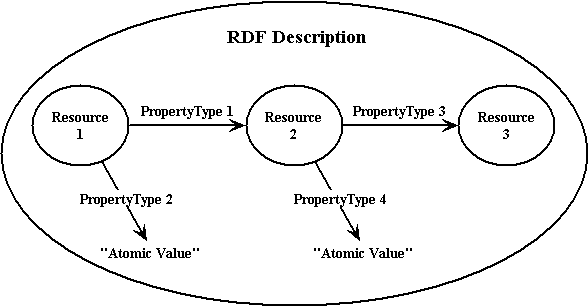
\includegraphics[width=8cm]{gfx/chapters/preliminaries/rdfdesc.png}
    \captionof{figure}{\textit{Resources} may have an atomic value or be linked other \textit{resources}.}
\end{center}

\section{Semantic Reasoner}
A semantic reasoner (also know as reasoning engine) or solely a reasoner, is a software which is capable of inferring logical results from an axioms set. The whole process also knows as entailment. The reasoning capability is crucially important since many applications developed for the Semantic Web \cite{parsia2004pellet}.

\begin{definition}[Rule of Inference]
In logic, a rule of inference (simply inference rule) is a logical structure composed of a function that exerts axioms, analyzes their syntax and generate a conclusion.
\end{definition}

\begin{definition}[OWL]
\ac{OWL} is designed for Semantic web-based applications that need to process and analyze the content of information rather of just displaying human readable information. OWL facilitates to machines the interpretability of data over the web. It also provide additional vocabulary with formal semantics. OWL has three dominant sub-languages: \textit{OWL Lite}, \textit{OWL DL} and \textit{OWL Full} \cite{mcguinness2004owl}.
\end{definition}
\subsection{OWL Horst}
OWL Horst is a subset of OWL Language, which is used by a rule reasoner engine to infer implicit information \cite{liu2016rors}.

\section{Big Data Analysis}
\subsection{Apache Hadoop}
\subsection{Apache Spark}
\subsubsection{Actions vs Trasformations}
\subsubsection{RDDs}
\section{SANSA Framework}
\ac{SANSA}\footnote{\url{http://sansa-stack.net/}} is an ongoing open-source\footnote{\url{https://github.com/SANSA-Stack}}  project to support scalability and expressiveness of semantic analytics. SANSA also provide enormous support of large-scale RDF datasets by a robust functional APIs. Sansa exploites the advantages of Apache Spark and Apache Flink to offer a solid backing of massive sized data sources in terms of data analysis \cite{lehmann2017distributed}.

\begin{center}
    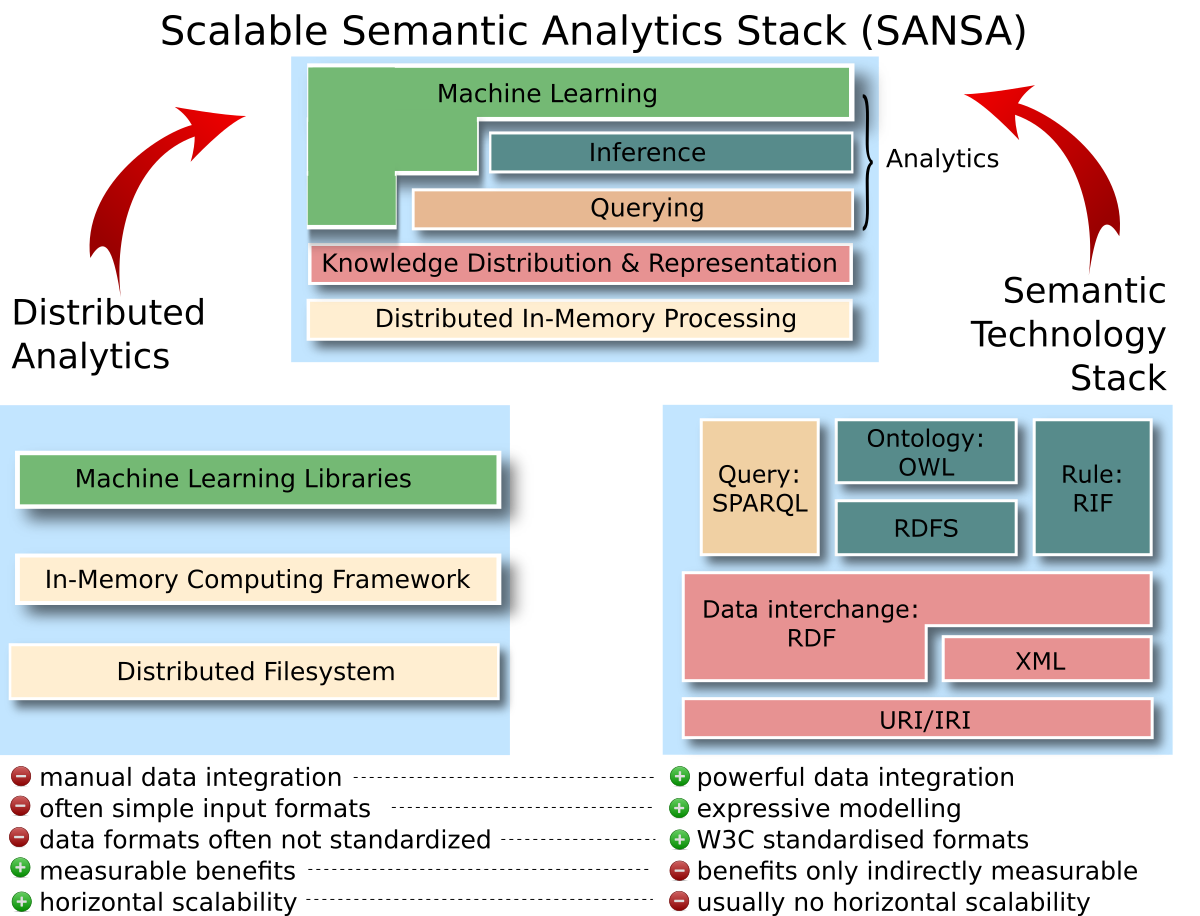
\includegraphics[width=10cm]{gfx/chapters/preliminaries/sansa1.png}
    \captionof{figure}{\ac{SANSA} Architecture.}
\end{center}



%*****************************************
%*****************************************
%*****************************************
%*****************************************
%*****************************************
